\documentclass{beamer}
\usepackage[utf8]{inputenc}
\usepackage{threeparttable}
%\usepackage{utopia} %font utopia imported

\usepackage{amsthm, booktabs, setspace, natbib, amsfonts,amssymb,epstopdf,textcomp,listings, xcolor}

\usepackage{adjustbox} % Shrink stuff
\usepackage{pgfpages}


\usepackage{tikz}
\usepackage{verbatim}
\setbeamertemplate{note page}{\pagecolor{yellow!5}\insertnote}
\usetikzlibrary{positioning}
\usetikzlibrary{snakes}
\usetikzlibrary{calc}
\usetikzlibrary{arrows}
\usetikzlibrary{decorations.markings}
\usetikzlibrary{shapes.misc}
\usetikzlibrary{matrix,shapes,arrows,fit,tikzmark}

\usepackage{amsmath}
\usepackage{mathpazo}
\usepackage{hyperref}
\usepackage{lipsum}
\usepackage{multimedia}
\usepackage{graphicx}
\usepackage{multirow}
\usepackage{dcolumn}
\usepackage{bbm}
\usepackage[space]{grffile}
\usepackage{tabularx}
\usepackage{subfig}
\usepackage{float}
\usepackage{multirow}

\usepackage{tabularx}
\usepackage{fancyhdr}
\usepackage{lscape}
\usepackage{mdframed}
\usepackage{mathtools}
\usepackage{array}

\usepackage{mwe}
\usepackage[skip=2pt,font=scriptsize]{caption}
\captionsetup{labelfont=bf, format=hang, labelsep=period, labelformat = empty}
%labelformat  =simple
%labelformat = empty

\usepackage{appendixnumberbeamer} %for avoid counting appendix slides add \appendix
\usepackage{colortbl}
\usepackage{xcolor}

%\usetheme{Warsaw}
\usetheme{Madrid}
\usecolortheme{default}



%------------------------------------------------------------
%This block of code defines the information to appear in the
%Title page
\title[Genetic Dilution in Improved Maize] %optional/
{A Case of Genetic Dilution in Improved Maize: Estimating
Comparative Advantage of Adoption in Ethiopia}


\author[et al]{Aleksandr Michuda \\ Cristina Chiarella \\Oscar Barriga-Cabanillas \\Juan Correa }


% \institute[UC Davis] % (optional)
% {
% %  \inst{1}%
%   Agricultural and Resource Economics\\
%   UC Davis
%  }

\date[January 2022] % (optional)
{CGIAR-SPIA \\
January, 2022}


%End of title page configuration block
%------------------------------------------------------------



%------------------------------------------------------------
%The next block of commands puts the table of contents at the 
%beginning of each section and highlights the current section:

\AtBeginSection[]
{
  \begin{frame}
    \frametitle{Table of Contents}
    \tableofcontents[currentsection]
  \end{frame}
}
%------------------------------------------------------------


\begin{document}

\setbeamertemplate{enumerate items}[square]
\setbeamercolor{item projected}{bg=none,fg=black}

%\setbeamercolor{enumerate items}{〈key=value〉 list} to
%\setbeamercolor{item projected}{bg=none,fg=beamer@blendedblue}

\setbeamertemplate{itemize items}[circle]
\setbeamercolor{itemize item}{fg=black}
\setbeamercolor{itemize subitem}{fg=black}

%%% TIKZ STUFF
\tikzset{   
        every picture/.style={remember picture,baseline},
        every node/.style={anchor=base,align=center,outer sep=1.5pt},
        every path/.style={thick},
        }
\newcommand\marktopleft[1]{%
    \tikz[overlay,remember picture] 
        \node (marker-#1-a) at (-.3em,.3em) {};%
}
\newcommand\markbottomright[2]{%
    \tikz[overlay,remember picture] 
        \node (marker-#1-b) at (0em,0em) {};%
}
\tikzstyle{every picture}+=[remember picture] 
\tikzstyle{mybox} =[draw=black, very thick, rectangle, inner sep=10pt, inner ysep=20pt]
\tikzstyle{fancytitle} =[draw=black,fill=red, text=white]
%%%% END TIKZ STUFF



%The next statement creates the title page.
\frame{\titlepage}

% %---------------------------------------------------------
% %This block of code is for the table of contents after
% %the title page
% \begin{frame}
% \frametitle{Table of Contents}
% \tableofcontents
% \end{frame}
% %---------------------------------------------------------




%---------------------------------------------------------
\begin{frame}
\frametitle{Research question}

Food security is a major challenge: Ethiopia is no exception

\begin{itemize}
    % \item Struggled to provide an adequate and reliable food supply
    \item Breakthroughs in maize germplasm ($\uparrow$ yields, $\uparrow$ drought tolerance)
\end{itemize}

However adoption of improved seed has remained a challenge

\begin{enumerate}[ {[}1{]} ]
    \item Market integration
    \item Access to supplementary inputs
    \item Agro-ecological considerations
\end{enumerate}

\textbf{We study how heterogeneity masks the true impact of adoption}

\begin{enumerate}[ {[}1{]} ]
    \item Explore heterogeneous comparative advantages through GRC: find puzzling no significant results.
    \item Compare definitions of improved seeds: self-reported, second generation or recycled, purity of genetic material, year of release, types and source.
    \item Low adoption of newer and purest varieties, which do return in higher yields. Poor farmers paying a premium for genetically diluted improved varieties.
\end{enumerate}

\end{frame}

%---------------------------------------------------------
\begin{frame}
\frametitle{Data}

\begin{itemize}
    % \item Struggled to provide an adequate and reliable food supply
    \item We focus on maize producing households 
    \item Self-reported use of improved seed varieties
    \item Compare self-reported and cropcut yields
\end{itemize}

\begin{figure}
    \centering
    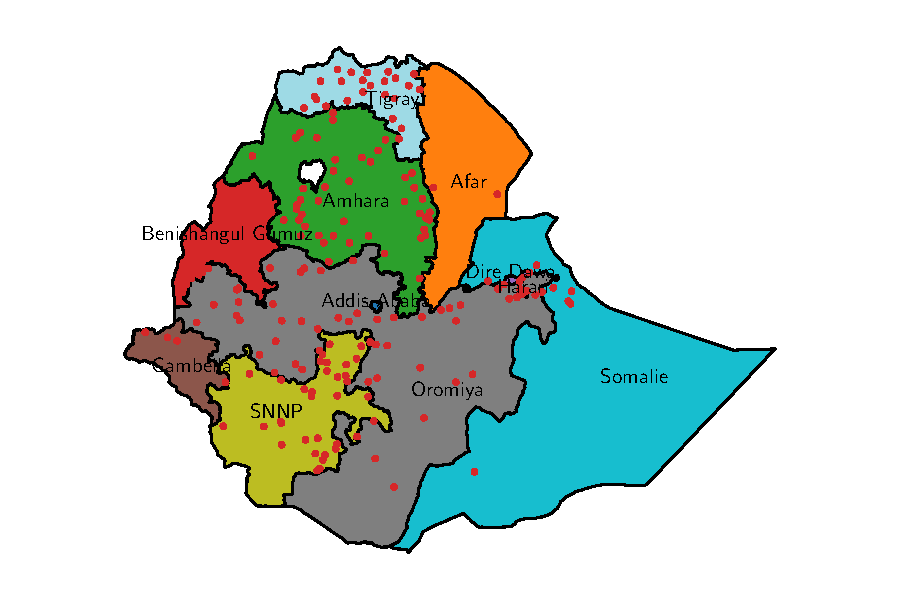
\includegraphics[scale=.4]{results/figures/map_hhids.pdf}
\end{figure}

% \textit{Add interesting image}
\end{frame}


%---------------------------------------------------------
\begin{frame}
\frametitle{Empirical Strategy I: Finding the returns from adoption}

\textbf{Understand the returns of adopting improved varieties: }
\begin{itemize}
    \item Some farmers have higher returns to adoption (comparative advantage)
    \item How comparative advantage plays a role on using improved seed varieties.
\end{itemize}  

% (Suri 2011; Tjernstr\"{o}m et al. 2020; Michler et al. 2019; Barriga et al. 2018)

We use a Correlated Random Coefficient Model:
\vspace{-2em}
\begin{center}
$$
    y_{it}= \delta + \Delta h_{it} + \theta_{i} + \phi\theta h_{it} + \tau_{i} + \epsilon_{it}
$$  
\end{center}

\begin{itemize}
    \item $y_{it}$: yields or profits for household i at time t
    \item $h$:  indicator for adoption
    \item $\tau$:  household’s absolute advantage
    \item \textbf{$\theta$: household’s comparative advantage}
    \item \textbf{$\Delta$: The marginal effect of adoption}
    \item $\phi$: Gains from adopting, relative to a household’s comparative advantage.
\end{itemize}

\end{frame}


%---------------------------------------------------------
\begin{frame}
\frametitle{Empirical Strategy I: Finding the returns from adoption}

Advantages:
\begin{enumerate}
    \item Identification does not rely on a IV 
    % (linear projection of observed adoption history)
    \item Disentangles absolute advantage from comparative advantage in adoption. ($\theta_i = \theta_A - \theta_N$)
\end{enumerate}

\begin{table}
\centering
\caption{Trajectories of Households}
\label{tbl:trajectories}
\begin{tabular}{lrr}
\toprule
Trajectory &  Frequency &    Share \\
\midrule
       000 &       2124 & 0.611927 \\
       111 &        456 & 0.131374 \\
       011 &        228 & 0.065687 \\
       001 &        219 & 0.063094 \\
       010 &        153 & 0.044080 \\
       100 &        108 & 0.031115 \\
       110 &         96 & 0.027658 \\
       101 &         87 & 0.025065 \\
\bottomrule
\multicolumn{3}{l}{Note: Table shows frequency and shares of each trajectory in sample. 1 denotes adoption and 0 otherwise. The first digit is for whether the household adopted in wave 1, the second digit for wave and the third digit for wave 3}
\end{tabular}
\end{table}


% Extending the model:

% \begin{itemize}
%     \item Implementing a nonparametric panel identification in a novel GRC (Group Random Coefficients)
%     \item Modeling and incorporating time-varying characteristics 
%     \item Complement ESS data with precipitation (CHIRPS) and temperature (CPC) data
% \end{itemize}  
\end{frame}


%---------------------------------------------------------
%---------------------------------------------------------
\begin{frame}
\frametitle{Empirical Strategy II: Returns to Different Types of Hybrid}
% \frametitle{Group Random Coefficients Results}
\textbf{Why farmers do \textit{(not)} adopt?}

\begin{enumerate}
    \item There are negative returns from adoption
    \item Comparative advantage is close to 0 unless you always adopt (perhaps driven by 
\end{enumerate}

\begin{figure}
    \centering
    \label{fig:traj_sum}
    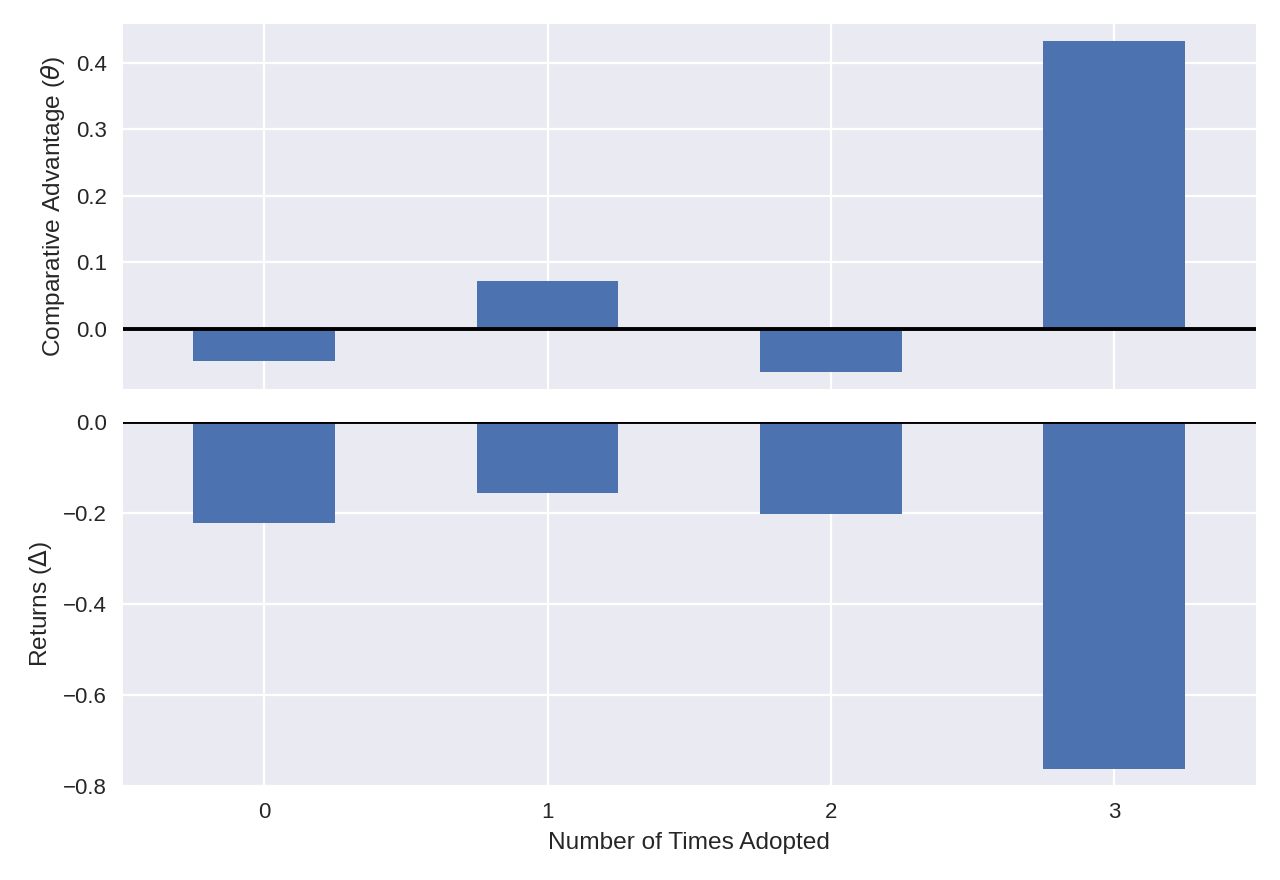
\includegraphics[scale=.4]{results/figures/traj_sum.png}
\end{figure}
 
\end{frame}

%---------------------------------------------------------

%---------------------------------------------------------
\begin{frame}
\frametitle{Endogenous Switching Regression Results}

Why do we see farmers adopting despite the seemingly small negative returns?

\begin{itemize}
    \item We use the DNA-fingerprinting to shed light on this puzzle
    \item DNA allows us to assess what varieties (and purity) farmers are using 
    \item Unfortunately, only available in the last round
\end{itemize}

We implement a switching regression approach

\end{frame}
%---------------------------------------------------------


%---------------------------------------------------------
\begin{frame}
\frametitle{Endogenous Switching Regression Results}

\begin{table}[H]
\resizebox{.5\textwidth}{!}{
\centering
\hspace*{-1.2cm}
\begin{threeparttable}
\caption{Effects on yields (log) from adopting improved maize varieties (DNA fingerprinting)}
\label{tab:switch2}
\begin{tabular}{l cccccc}
\hline
\hline
            &Adopters yields&Non-adopters yields&         ATE&          SE&     p-value\\
\hline
\textit{DNA 70, SR yields}&            &            &            &            &            \\
ATT         &        7.17&        7.31&       -0.14&       0.026&      0.0000\\
%
%
%
ATU         &        8.76&        6.76&        2.00&       0.036&      0.0000\\
%
%
%
\textit{DNA 90, SR yields}&            &            &            &            &            \\
ATT         &        7.18&        9.07&       -1.90&       0.023&      0.0000\\
%
%
%
ATU         &        7.01&        6.80&        0.21&       0.022&      0.0000\\
%
%
%
\textit{DNA 95, SR yields}&            &            &            &            &            \\
ATT         &        7.30&        7.08&        0.22&       0.036&      0.0000\\
%
%
%
ATU         &        6.87&        6.86&       0.018&       0.029&      0.5496\\
%
%
%
\textit{HYB, SR yields}&            &            &            &            &            \\
ATT         &        7.28&        7.25&       0.030&       0.028&      0.2892\\
%
%
%
ATU         &        7.06&        6.85&        0.21&       0.028&      0.0000\\
%
%
%
\textit{DTMZ, SR yields}&            &            &            &            &            \\
ATT         &        7.42&        6.53&        0.89&       0.074&      0.0000\\
%
%
%
ATU         &        7.11&        7.02&       0.089&       0.022&      0.0001\\
%
%
%
\textit{CGIAR source, SR yields}&            &            &            &            &            \\
ATT         &        7.13&        6.71&        0.43&       0.033&      0.0000\\
%
%
%
ATU         &        9.19&        6.89&        2.31&       0.018&      0.0000\\
%
%
%
\textit{Year 2010+, SR yields}&            &            &            &            &            \\
ATT         &        7.44&        6.92&        0.53&       0.039&      0.0000\\
%
%
%
ATU         &        8.98&        6.91&        2.07&       0.056&      0.0000\\
%
%
%
\hline
\hline
\end{tabular}

\begin{tablenotes}
\footnotesize
\item{Note: Full set of controls include: parcel size (in HA), household labor, hired labor, fertilizer costs, other input costs irrigation (dummy), mechanization (dummy), organic fertilizer (dummy). Instruments for the adoption equation include: years of education of hh head, age of hh head, female head, land title, asset index, seed costs. All results include full set of controls. DNA 70, 90 and 95 refer to improved varieties defined by DNA finerprinting with purity levels of 70, 90 and 95\%, respectively. HYB equals 1 for a hybrid variety, 0 for an open-pollinated variety. DTMZ equals 1 for a Drought-tolerant maize variety}
\end{tablenotes}
\end{threeparttable}
}
\end{table}


 
\end{frame}
%---------------------------------------------------------

%---------------------------------------------------------
\begin{frame}
\frametitle{Discussion}
Negative and small returns to adoption from self-reported improved varieties.
\begin{itemize}
    \item But positive returns to more genetically pure, DTMZ, CG- sourced and newer varieties.
    \item All DNA fingerprints are 70\% pure or higher. Control group has high share of false positives: no proper control. 
    
\end{itemize}
Negative GRC results mask a large heterogeneity in returns to adoption. 
\begin{itemize}
    \item Low purchase of newly bred hybrids, diluted DNA, low inputs use.
 
\end{itemize}  

Effects of high-yielding varieties diminishes over time, but traditional varieties are well adapted to local agro-ecological conditions.

\begin{itemize}
    \item There may be a threshold in time above which it may be more profitable to use a traditional variety than an improved one that has been around for too many generations. 

\end{itemize}


\end{frame}

%---------------------------------------------------------
\begin{frame}{}
    Thank you!
\end{frame}

\begin{frame}{Raw Trajectories}
    \begin{figure}
        \centering
        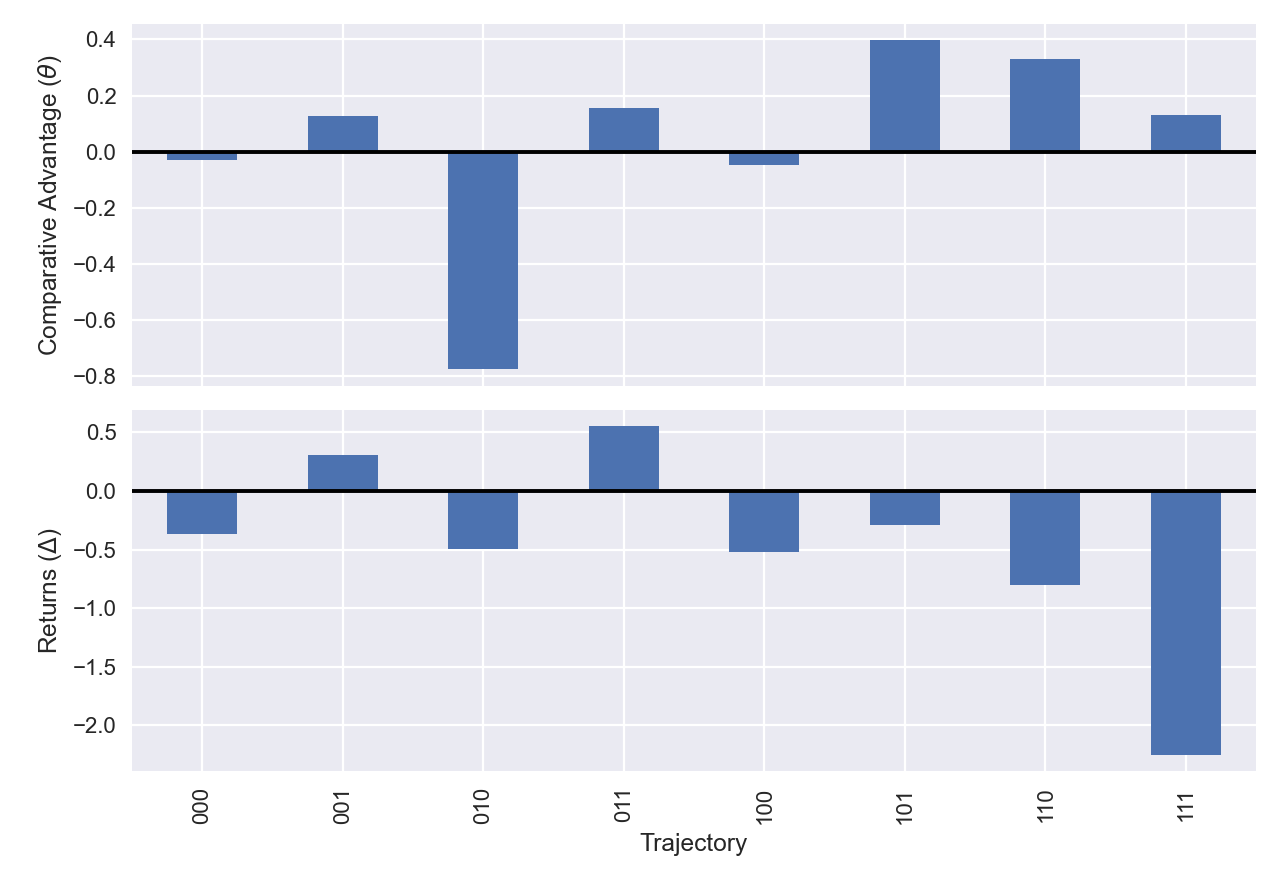
\includegraphics[scale=.5]{results/figures/theta.png}
    \end{figure}
\end{frame}


\bibliography{references}

\end{document}